%\appendix
%{\bfseries \huge Constraining torus models for AGN using X-ray observations}

\chapter{This is another appendix}

%\begin{center}
%  {\it ``You could put an introductionary text here''} \\
%  \vspace{1cm}
%\end{center}

\section{$X(\tau)$ for all sources} \label{appendix_lightcurves}
In this Appendix we show for each source in the Andonie sample from Chapter~\ref{ch:gas_distribution} the detailed trends of $X$ as a function of the delay/smoothing $\tau$ (Eq.~\ref{eq:X_tau}) as determined by our simulations. We remind the reader that $X=0$ is our best estimate of the reprocessor size, while $X=\pm 1$ are $1\sigma$ equivalent upper and lower limits (68.3\% probability range).

\begin{figure}
\begin{center}
    {
  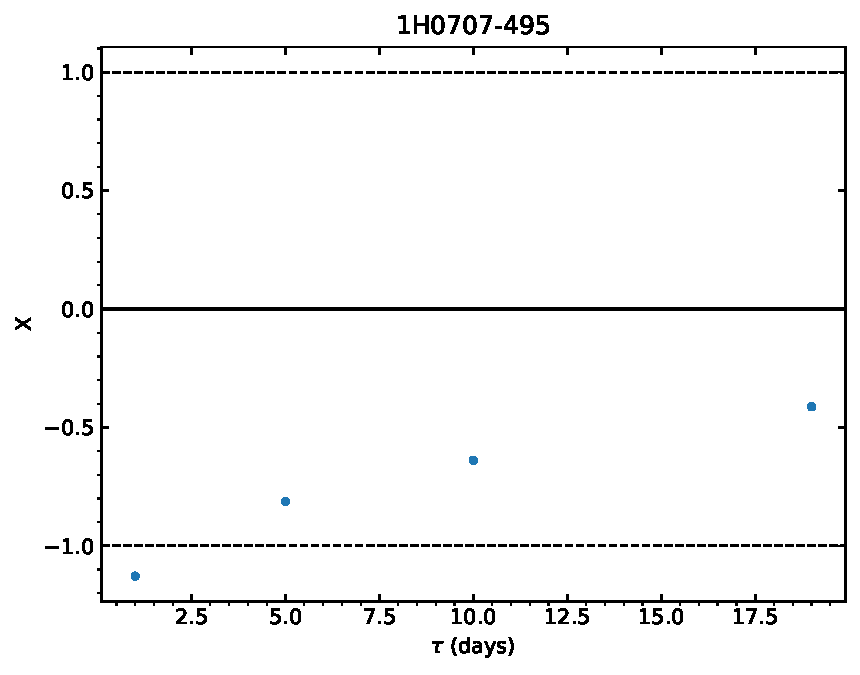
\includegraphics[width=0.49\textwidth]{Figs/Chapter5/X_tau/X_tau_1H0707-495.pdf}  \hfill
  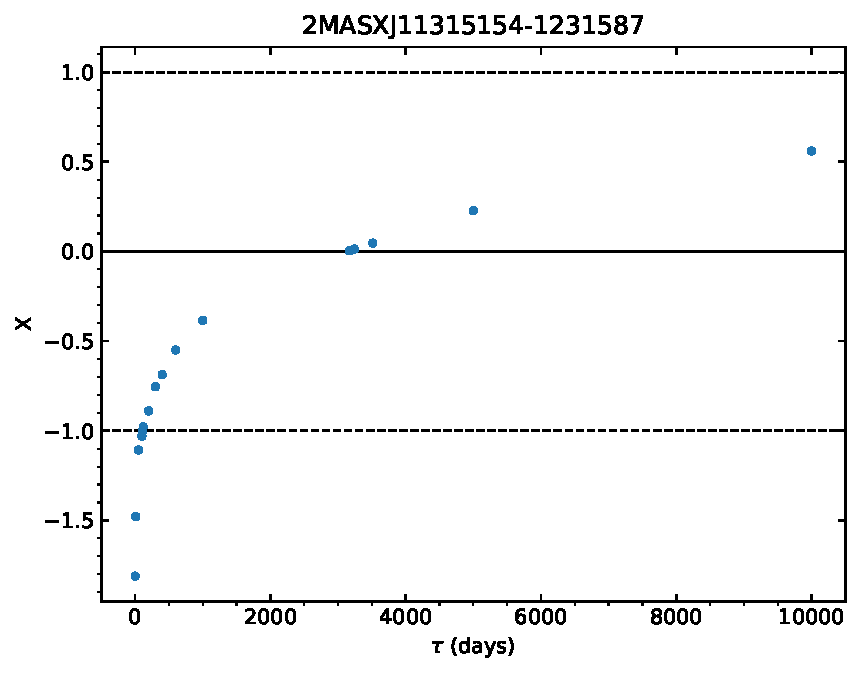
\includegraphics[width=0.49\textwidth]{Figs/Chapter5/X_tau/X_tau_2MASXJ11315154-1231587.pdf} \\
  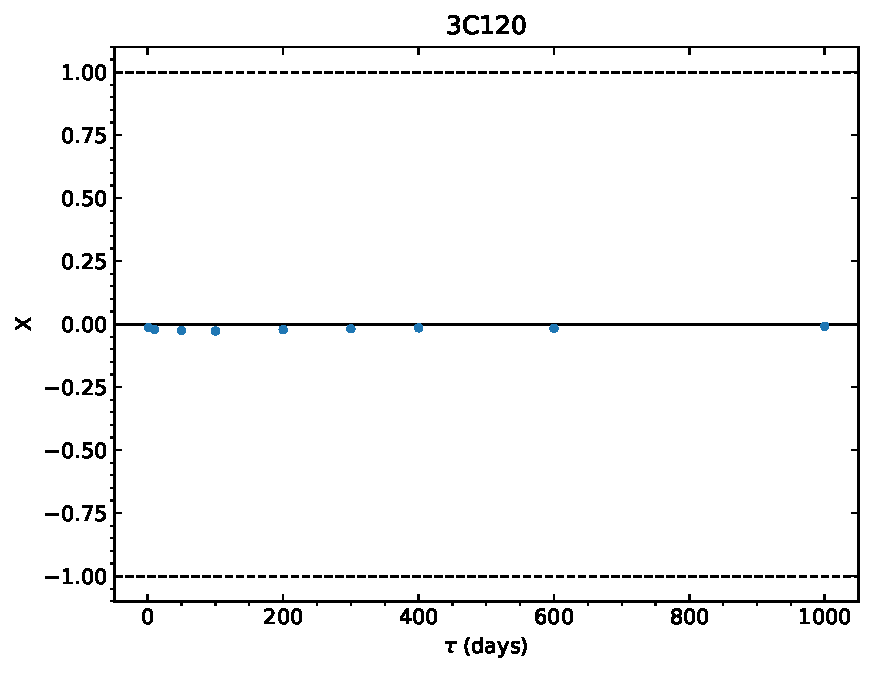
\includegraphics[width=0.49\textwidth]{Figs/Chapter5/X_tau/X_tau_3C120.pdf} \hfill 
  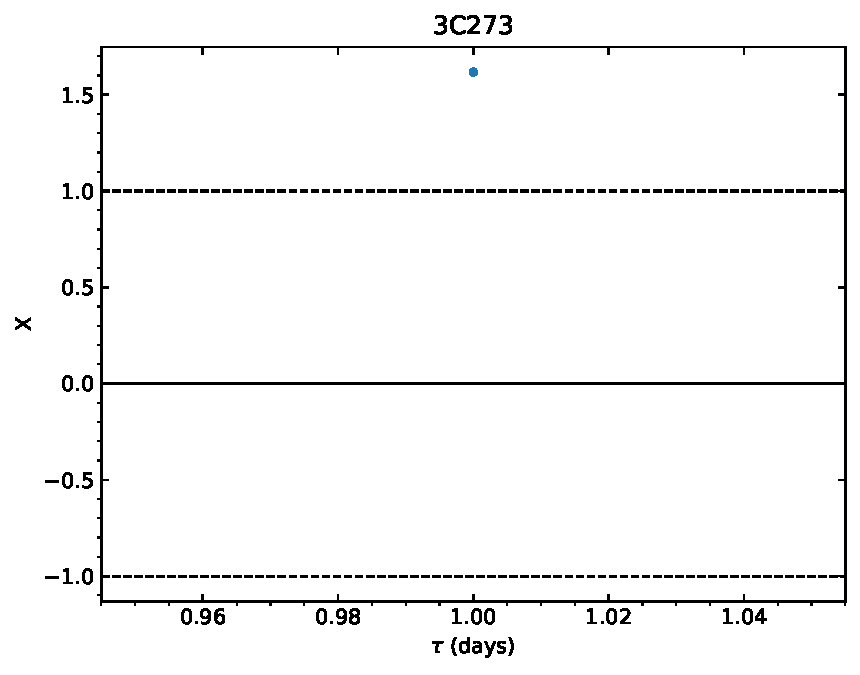
\includegraphics[width=0.49\textwidth]{Figs/Chapter5/X_tau/X_tau_3C273.pdf} \hfill \\
  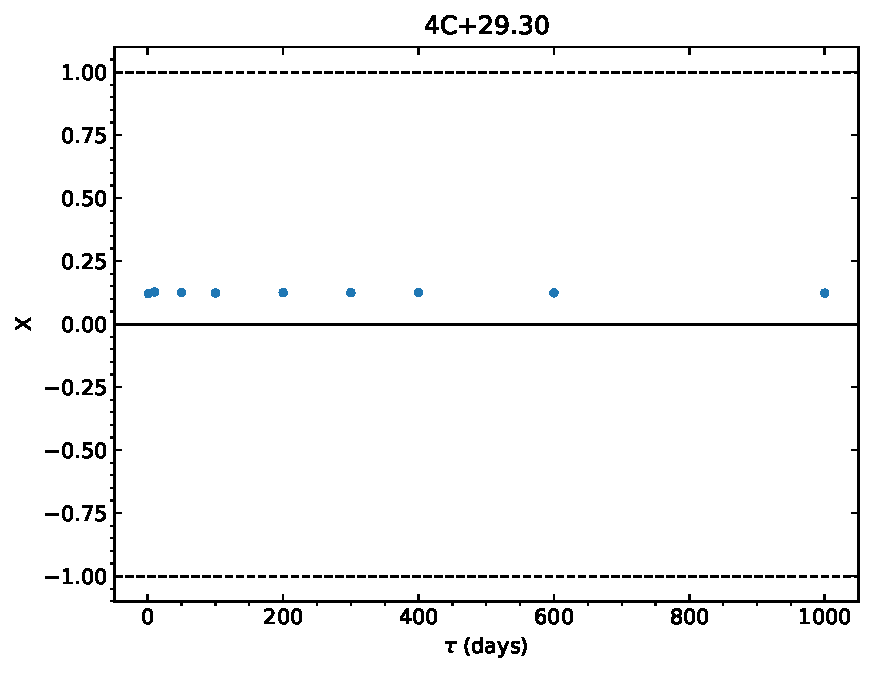
\includegraphics[width=0.49\textwidth]{Figs/Chapter5/X_tau/X_tau_4C+29.30.pdf} \hfill 
  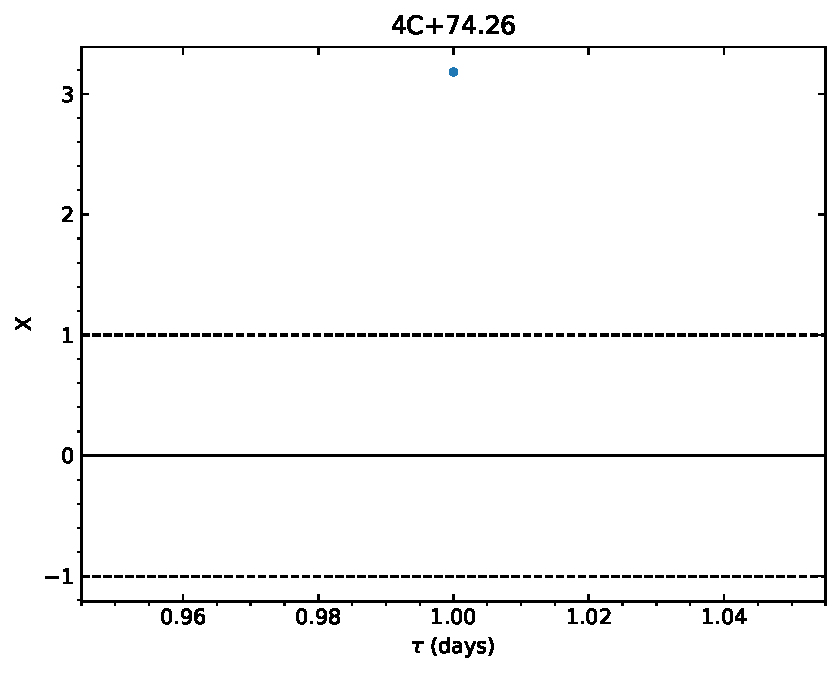
\includegraphics[width=0.49\textwidth]{Figs/Chapter5/X_tau/X_tau_4C+74.26.pdf} \hfill \\
  \caption{X$(\tau)$ for the galaxy sample from Andonie et al. in prep. Best estimate of the reprocessor size (X$=0$) is shown as a black solid line, while upper and lower limits (X$=\pm1$) are shown as dashed lines}
    \label{fig:Xtau_1}
  }
\end{center}
\end{figure}

\begin{figure}
\begin{center}
    {
  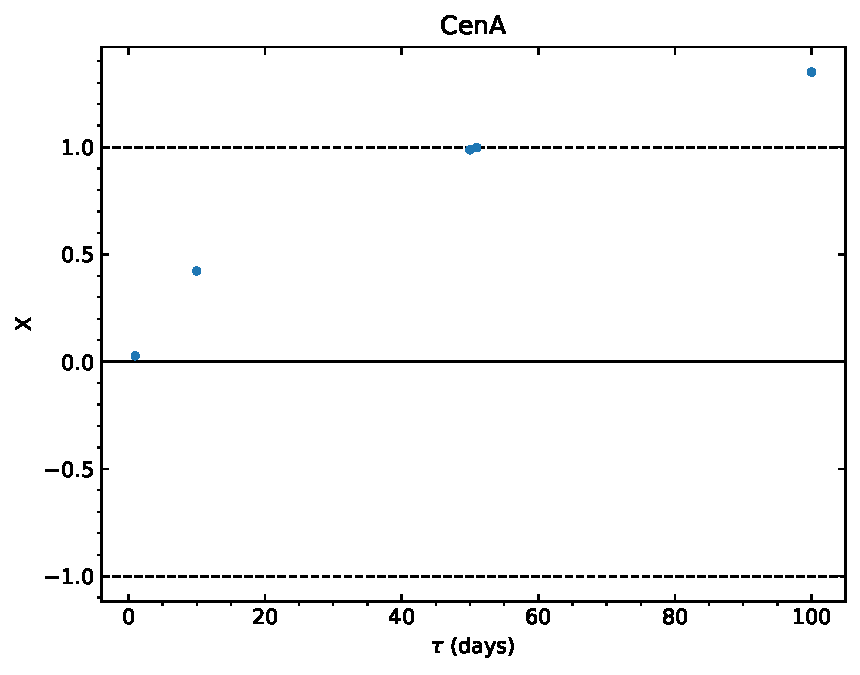
\includegraphics[width=0.49\textwidth]{Figs/Chapter5/X_tau/X_tau_CenA.pdf} \hfill 
  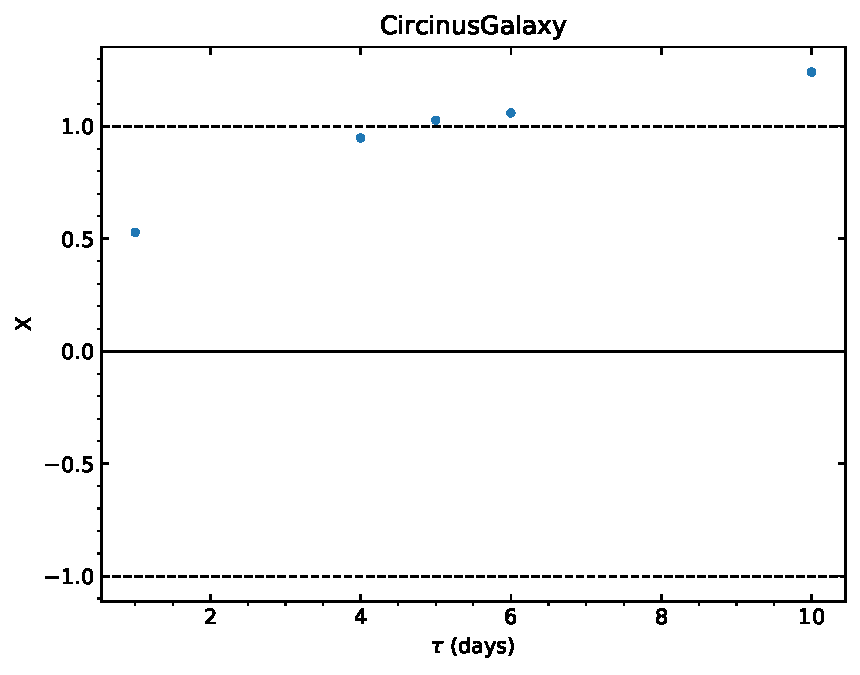
\includegraphics[width=0.49\textwidth]{Figs/Chapter5/X_tau/X_tau_CircinusGalaxy.pdf} \hfill \\
  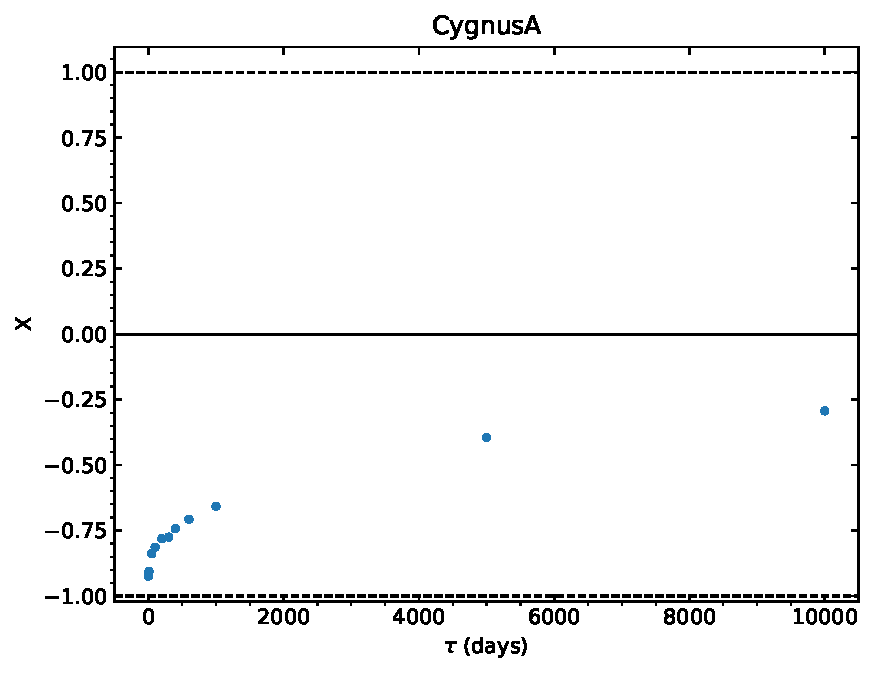
\includegraphics[width=0.49\textwidth]{Figs/Chapter5/X_tau/X_tau_CygnusA.pdf} \hfill 
  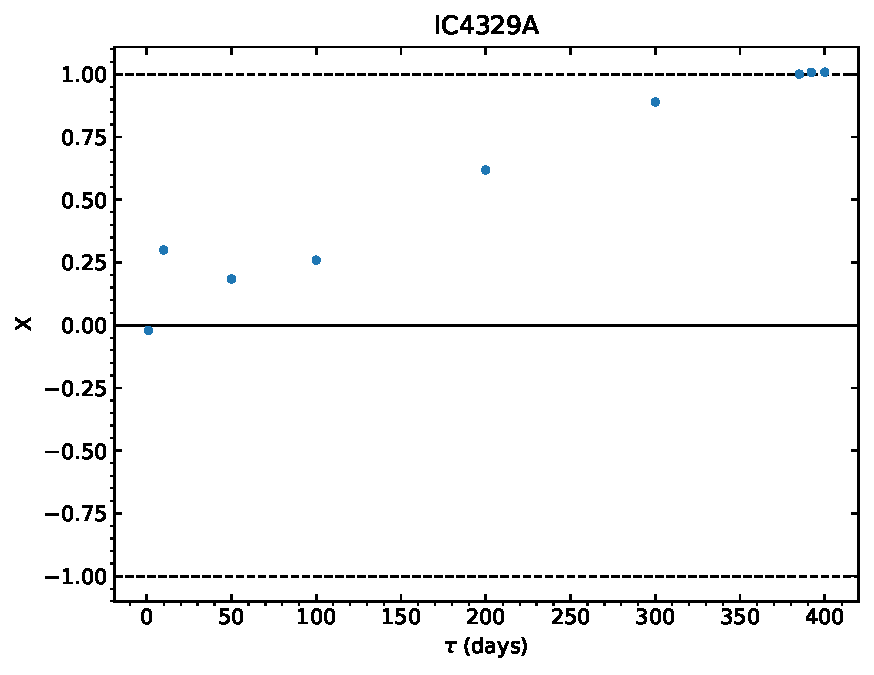
\includegraphics[width=0.49\textwidth]{Figs/Chapter5/X_tau/X_tau_IC4329A.pdf} \hfill \\
  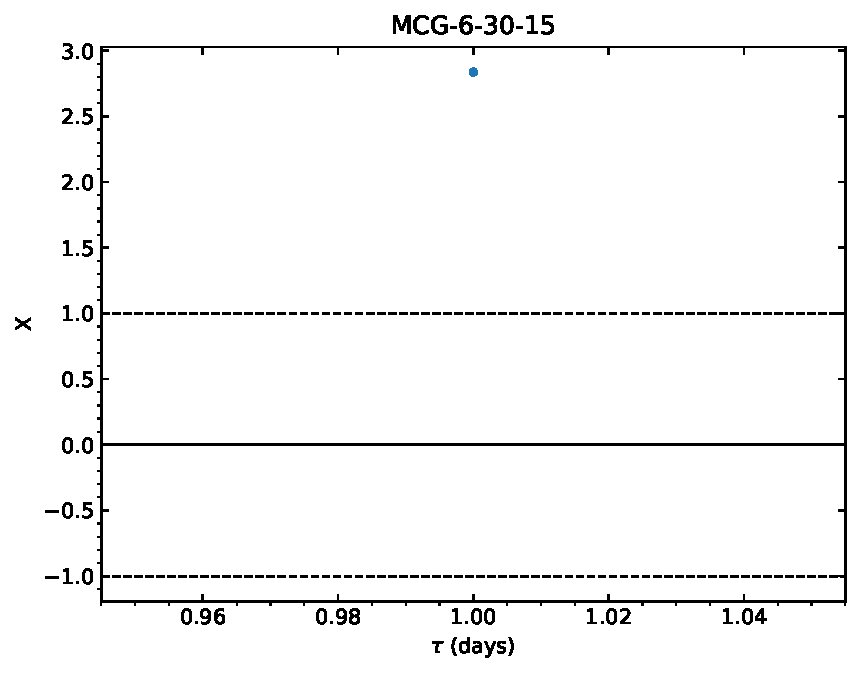
\includegraphics[width=0.49\textwidth]{Figs/Chapter5/X_tau/X_tau_MCG-6-30-15.pdf} \hfill 
  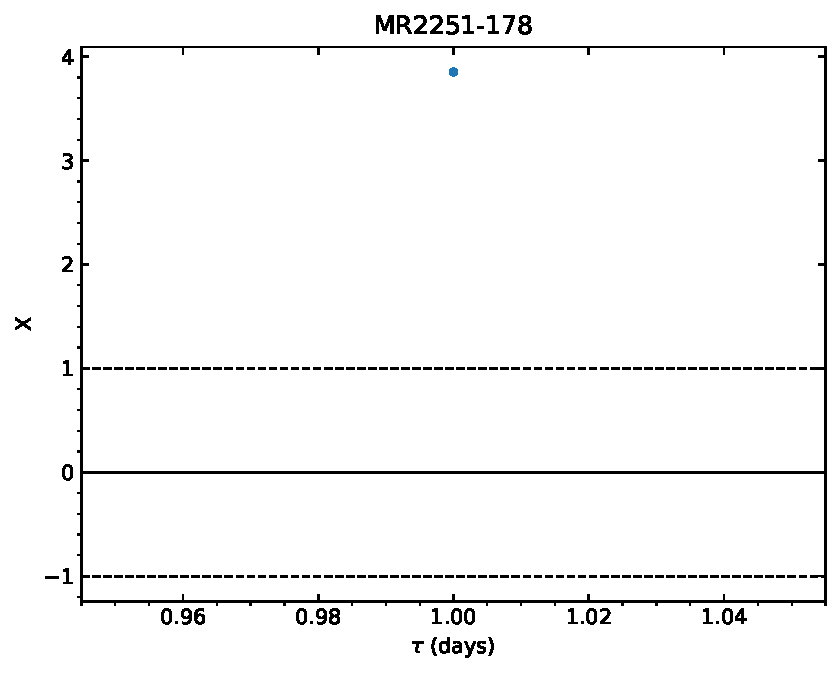
\includegraphics[width=0.49\textwidth]{Figs/Chapter5/X_tau/X_tau_MR2251-178.pdf} \hfill \\
  \caption{Fig.~\ref{fig:Xtau_1} continued.}
    \label{fig:Xtau_2}
  }
\end{center}
\end{figure}

\begin{figure}
\begin{center}
    {
  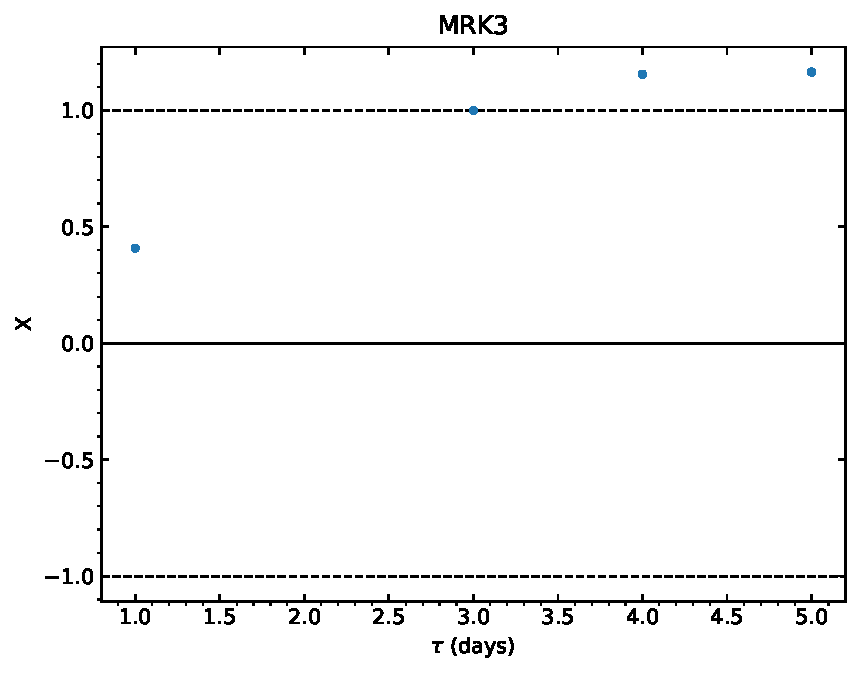
\includegraphics[width=0.49\textwidth]{Figs/Chapter5/X_tau/X_tau_MRK3.pdf} \hfill 
  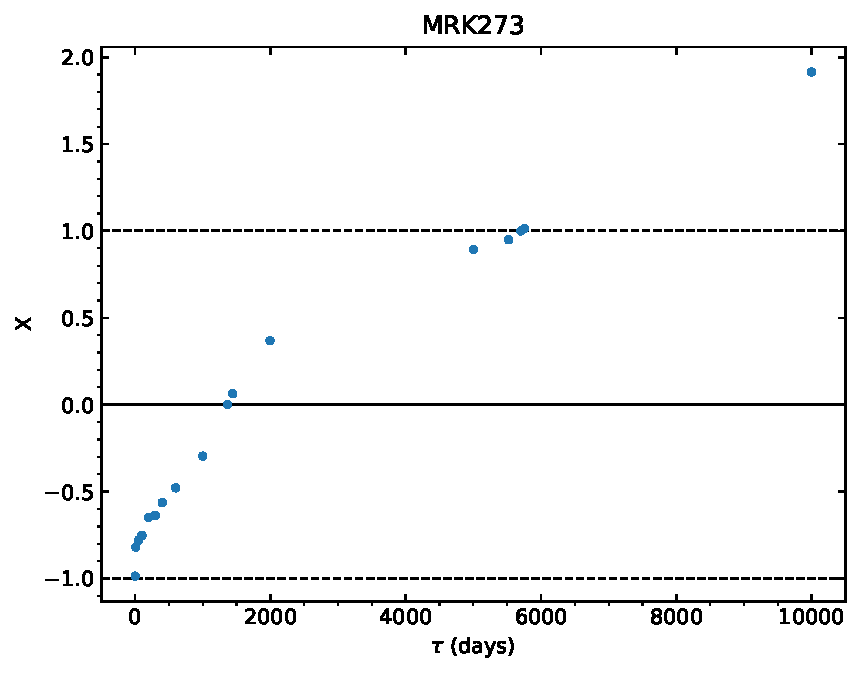
\includegraphics[width=0.49\textwidth]{Figs/Chapter5/X_tau/X_tau_MRK273.pdf} \hfill \\
  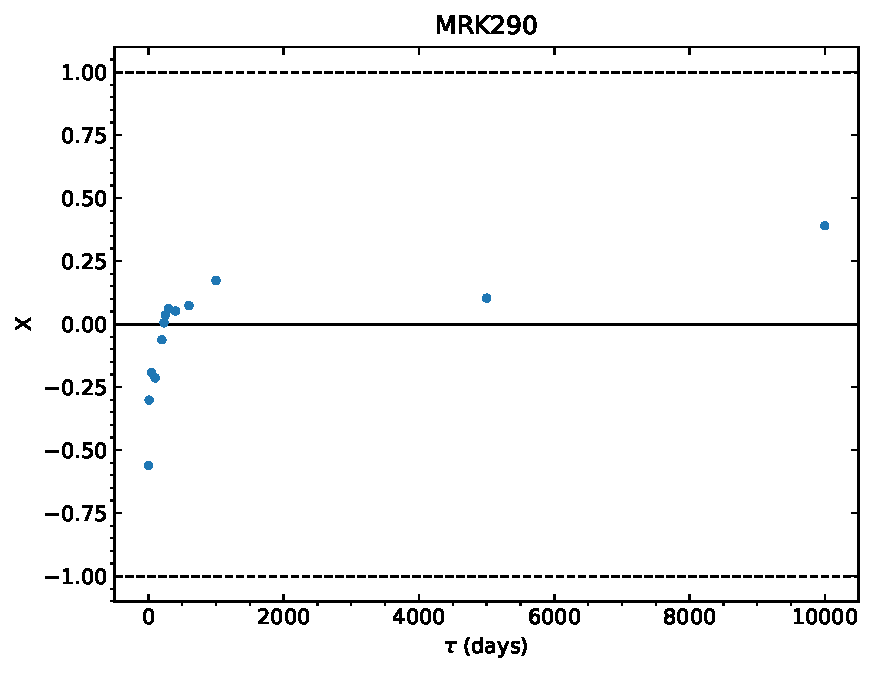
\includegraphics[width=0.49\textwidth]{Figs/Chapter5/X_tau/X_tau_MRK290.pdf} \hfill 
  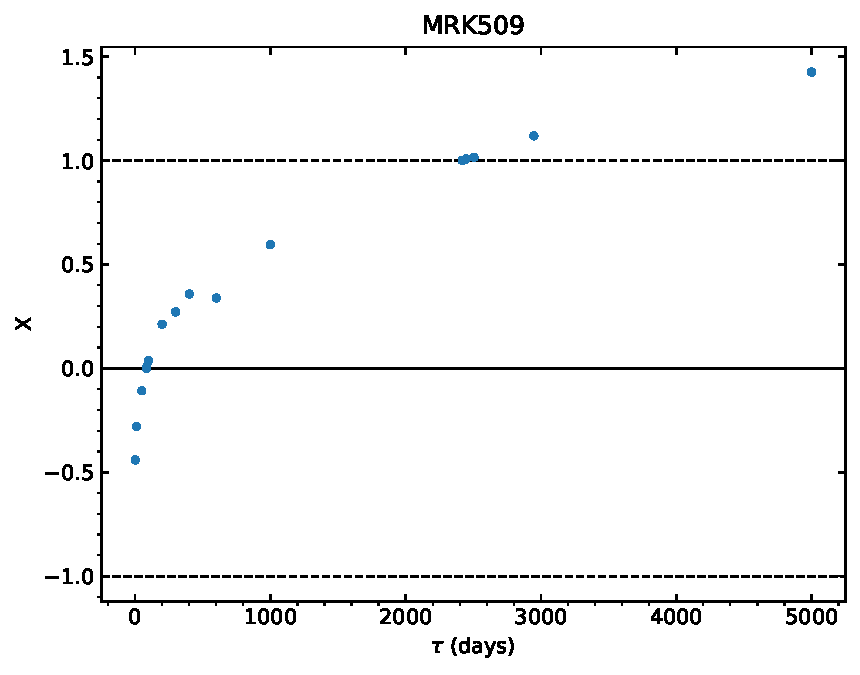
\includegraphics[width=0.49\textwidth]{Figs/Chapter5/X_tau/X_tau_MRK509.pdf}  \\
  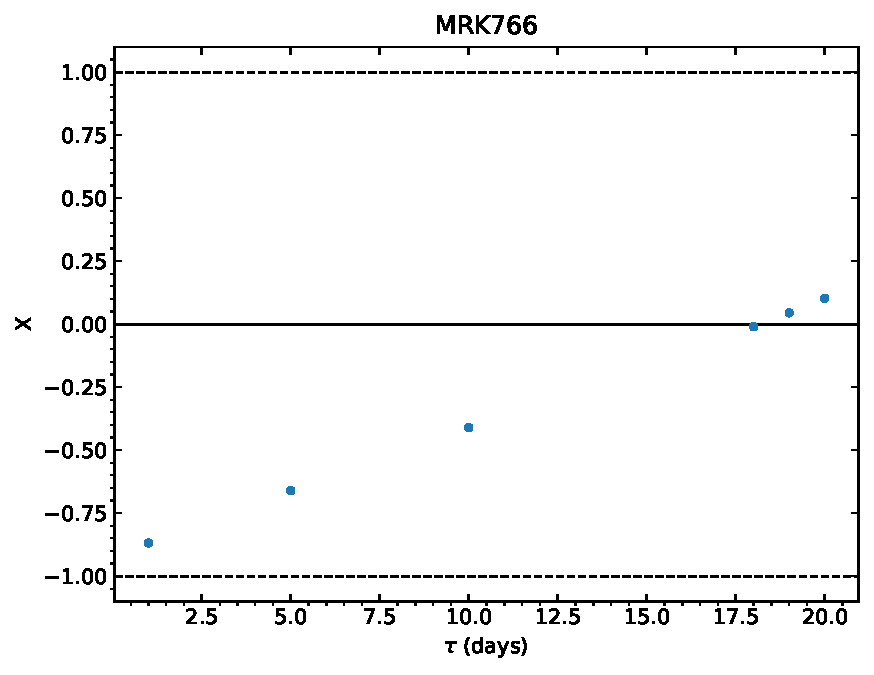
\includegraphics[width=0.49\textwidth]{Figs/Chapter5/X_tau/X_tau_MRK766.pdf}  \hfill 
  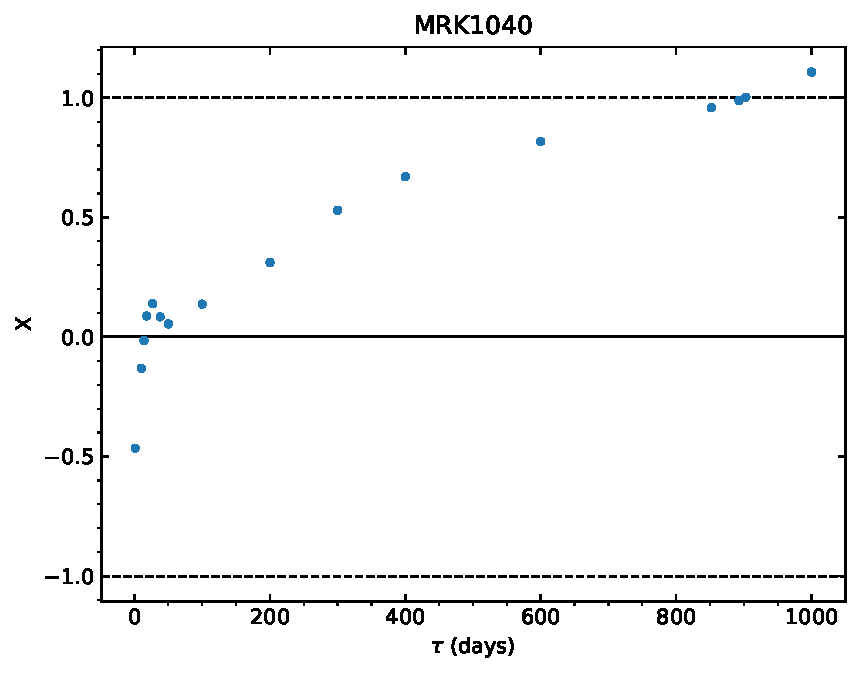
\includegraphics[width=0.49\textwidth]{Figs/Chapter5/X_tau/X_tau_MRK1040.pdf} \\
  \caption{Fig.~\ref{fig:Xtau_1} continued.}
    \label{fig:Xtau_3}
  }
\end{center}
\end{figure}

\begin{figure}
\begin{center}
    {
  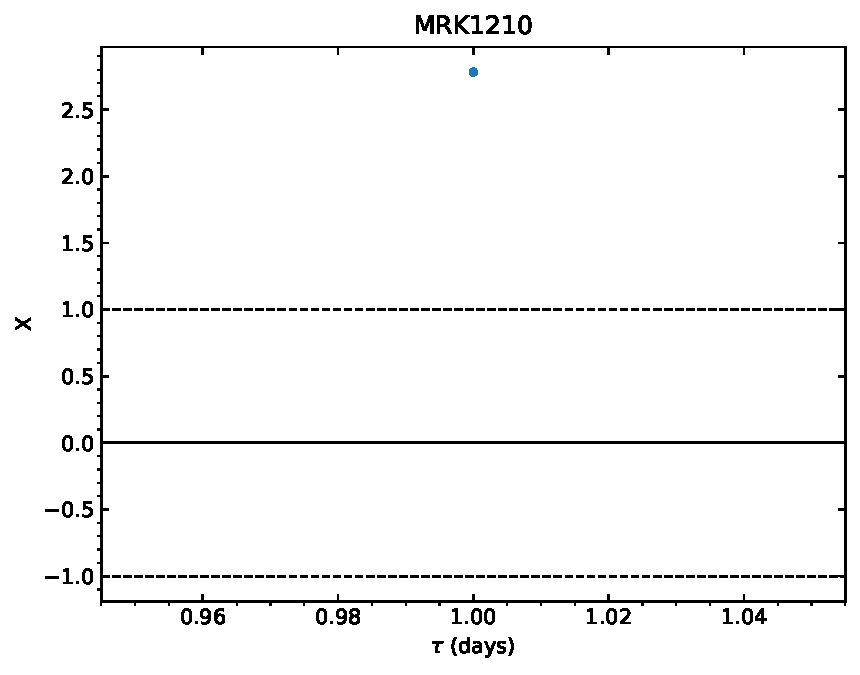
\includegraphics[width=0.49\textwidth]{Figs/Chapter5/X_tau/X_tau_MRK1210.pdf} \hfill
  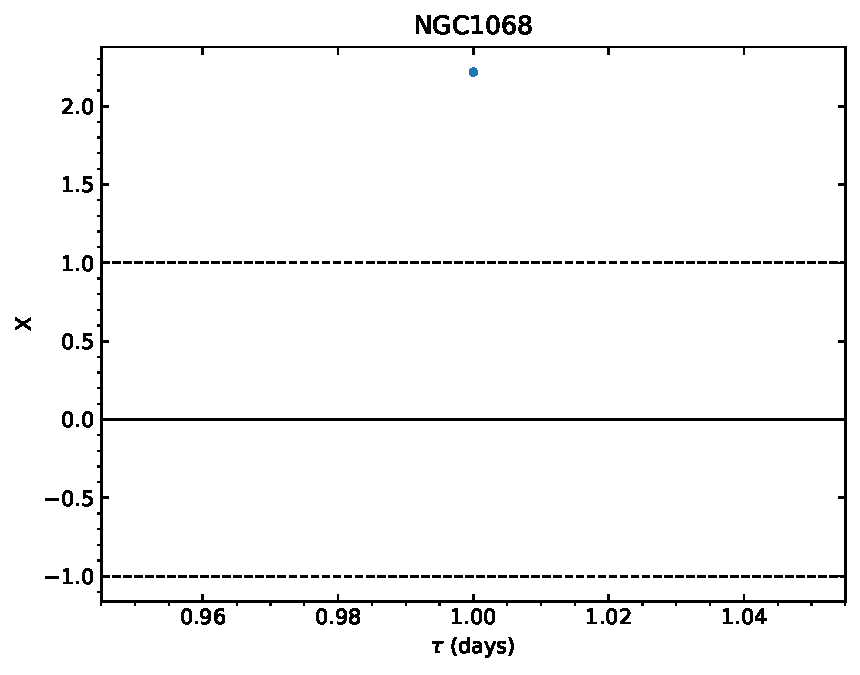
\includegraphics[width=0.49\textwidth]{Figs/Chapter5/X_tau/X_tau_NGC1068.pdf} \\
  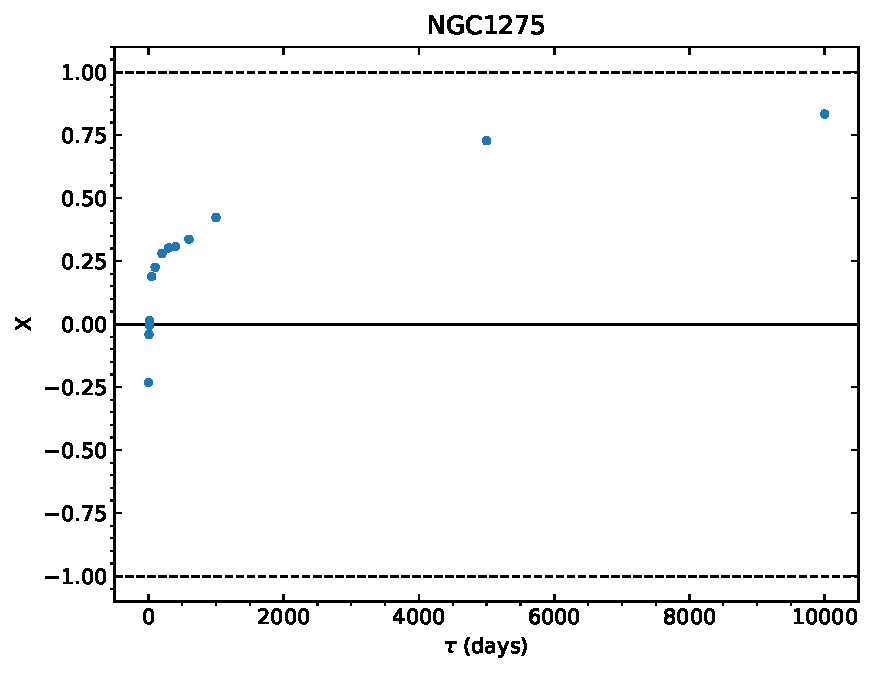
\includegraphics[width=0.49\textwidth]{Figs/Chapter5/X_tau/X_tau_NGC1275.pdf} \hfill 
  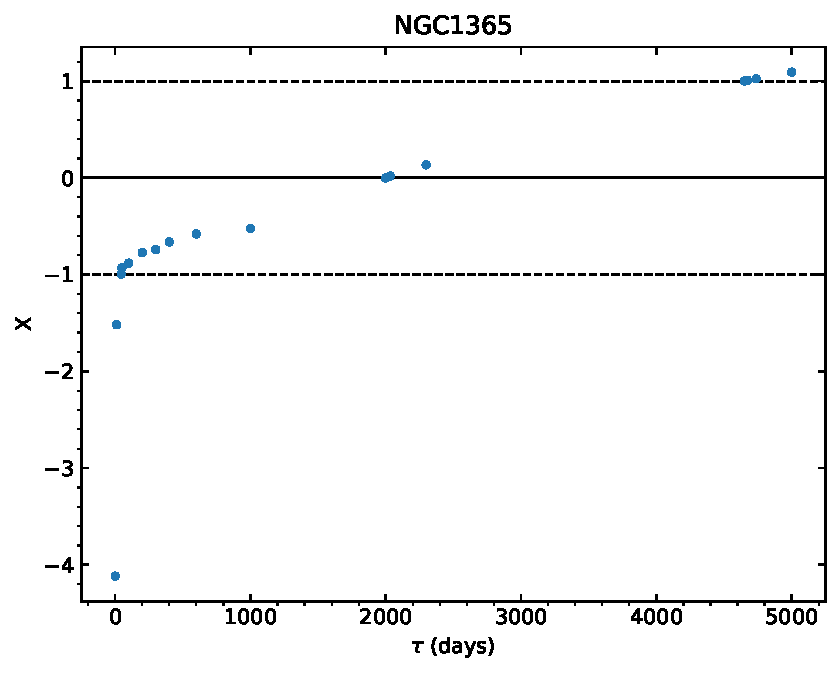
\includegraphics[width=0.49\textwidth]{Figs/Chapter5/X_tau/X_tau_NGC1365.pdf} \\
  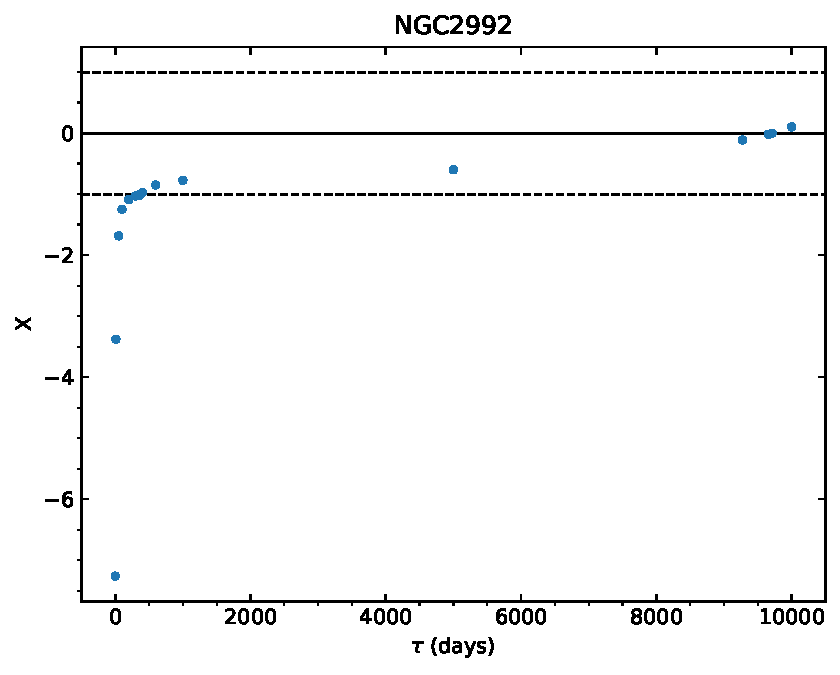
\includegraphics[width=0.49\textwidth]{Figs/Chapter5/X_tau/X_tau_NGC2992.pdf}  \hfill
  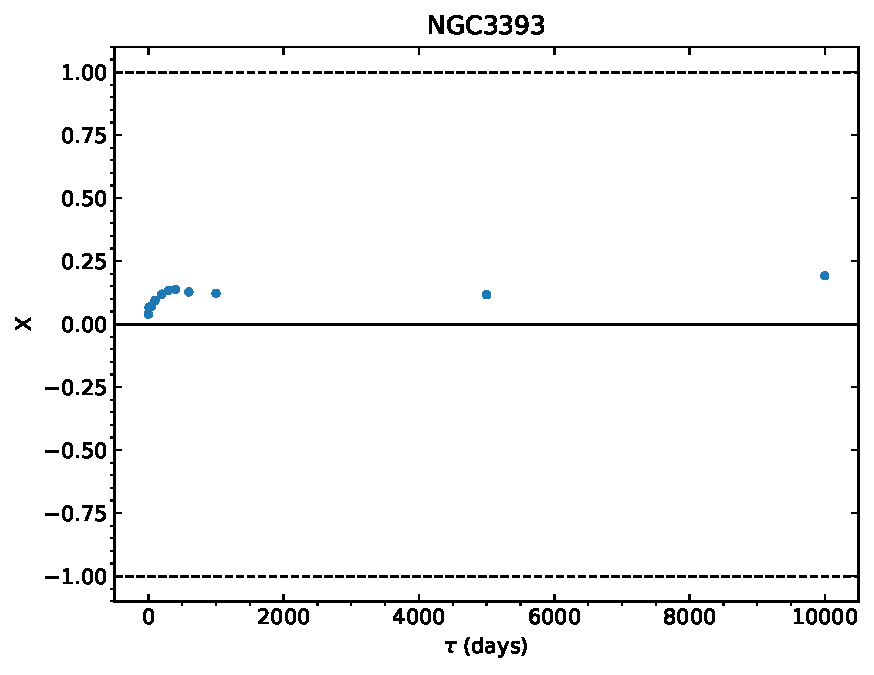
\includegraphics[width=0.49\textwidth]{Figs/Chapter5/X_tau/X_tau_NGC3393.pdf}  \hfill
  \caption{Fig.~\ref{fig:Xtau_1} continued.}
    \label{fig:Xtau_4}
  }
\end{center}
\end{figure}

\begin{figure}
\begin{center}
    {
  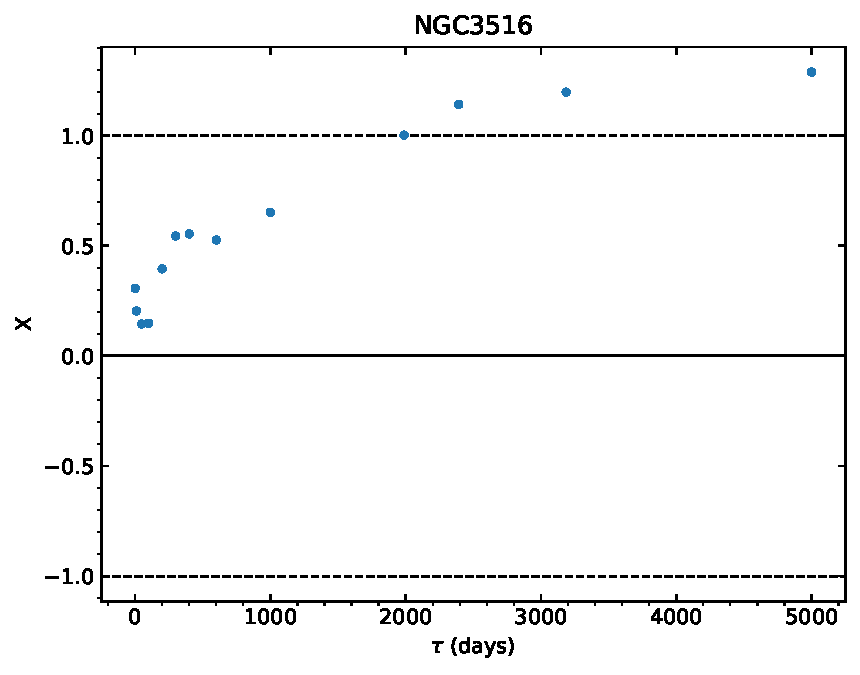
\includegraphics[width=0.49\textwidth]{Figs/Chapter5/X_tau/X_tau_NGC3516.pdf}
  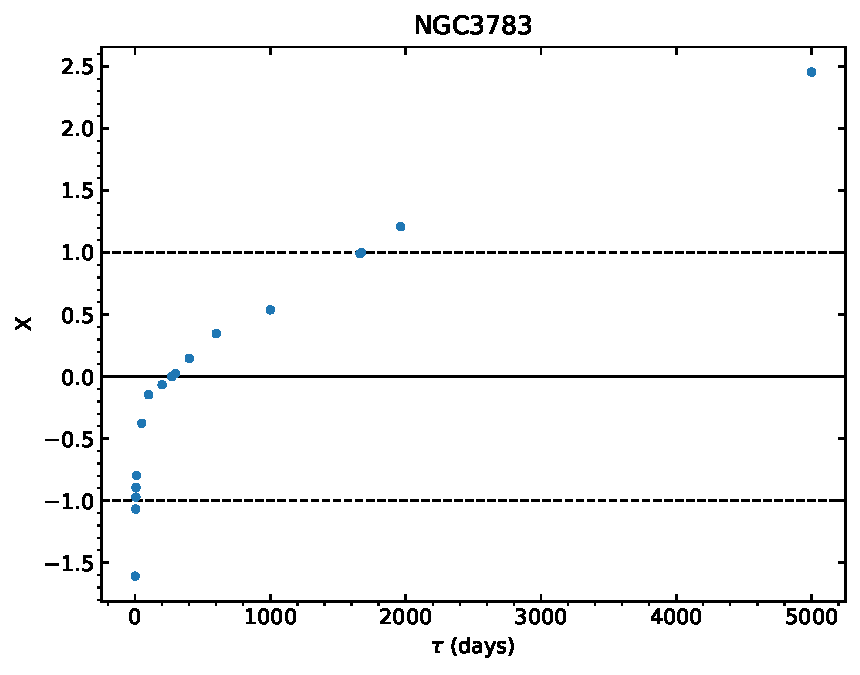
\includegraphics[width=0.49\textwidth]{Figs/Chapter5/X_tau/X_tau_NGC3783.pdf} \hfill  \\
  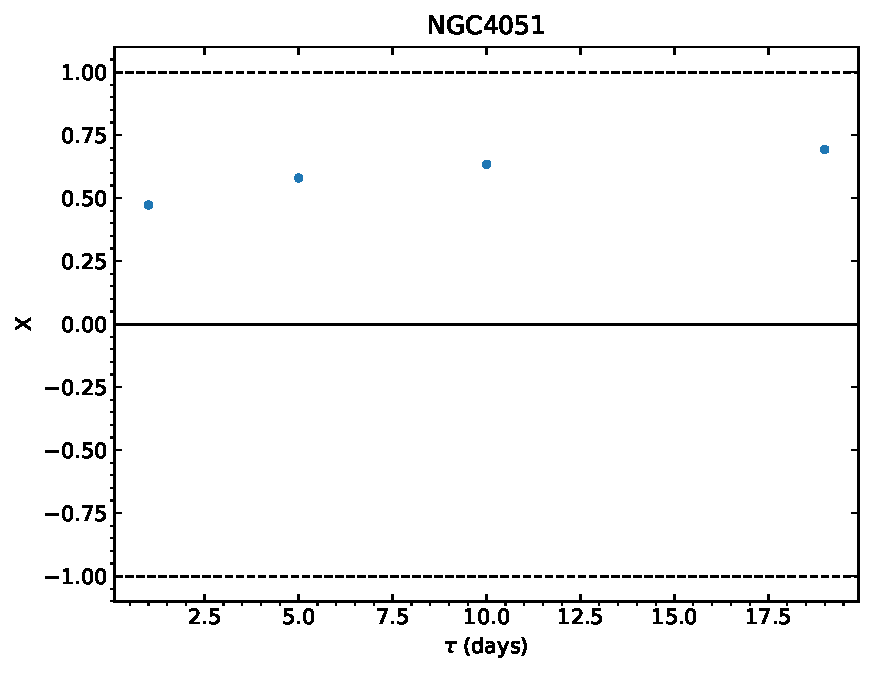
\includegraphics[width=0.49\textwidth]{Figs/Chapter5/X_tau/X_tau_NGC4051.pdf}  
  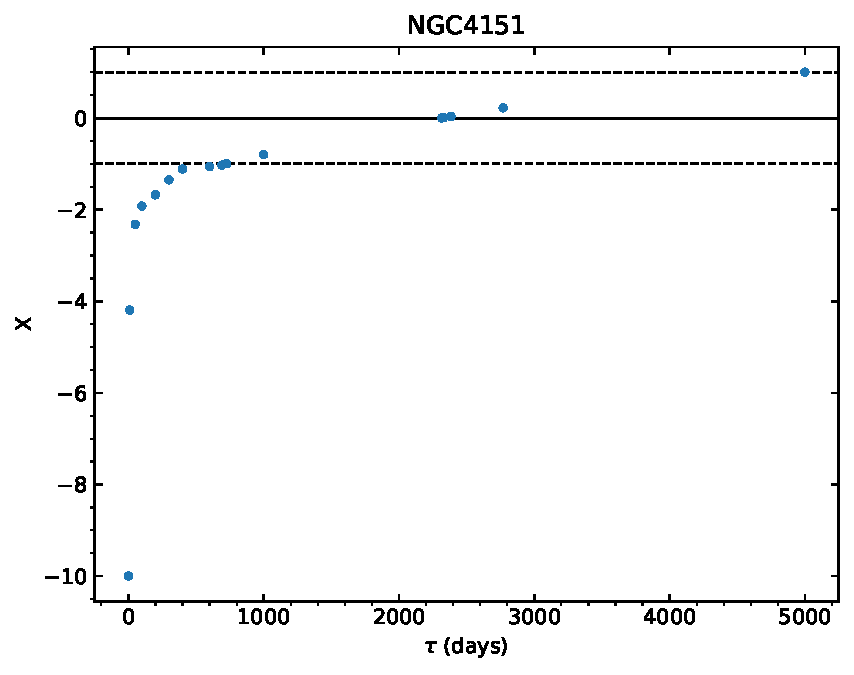
\includegraphics[width=0.49\textwidth]{Figs/Chapter5/X_tau/X_tau_NGC4151.pdf}  \hfill \\
  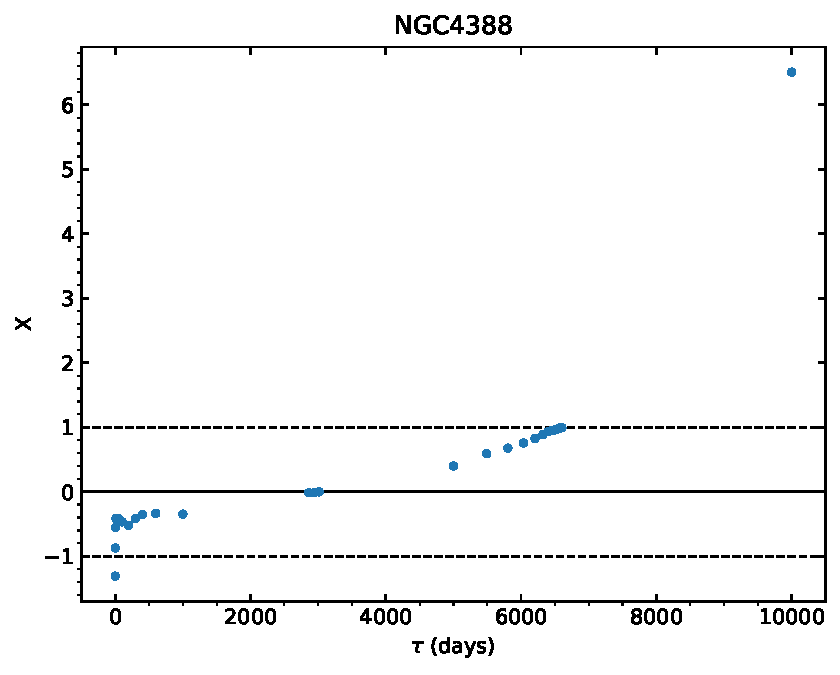
\includegraphics[width=0.49\textwidth]{Figs/Chapter5/X_tau/X_tau_NGC4388.pdf} 
  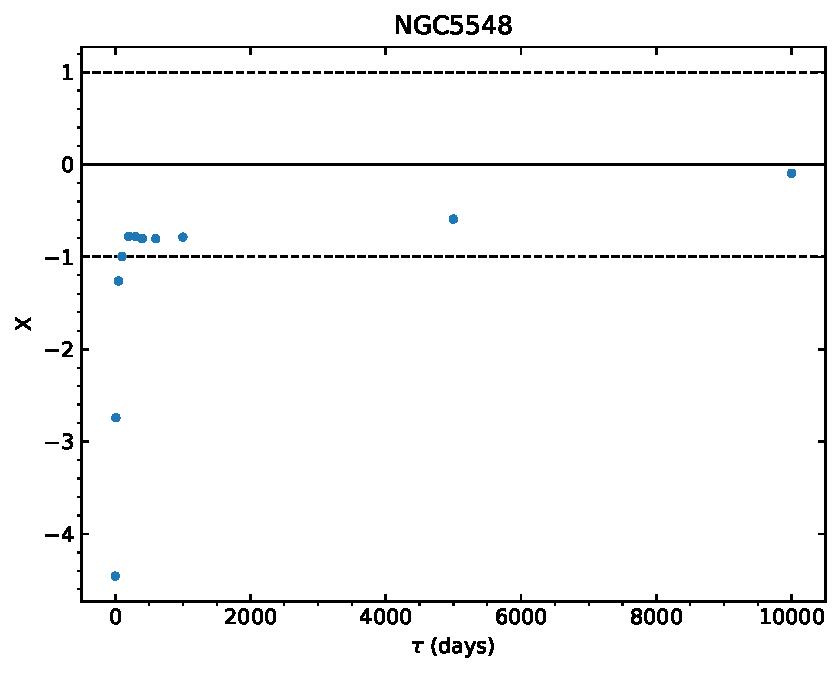
\includegraphics[width=0.49\textwidth]{Figs/Chapter5/X_tau/X_tau_NGC5548.pdf} \hfill 
  \caption{Fig.~\ref{fig:Xtau_1} continued.}
    \label{fig:Xtau_5}
  }
\end{center}
\end{figure}

\begin{figure}
\begin{center}
    {
  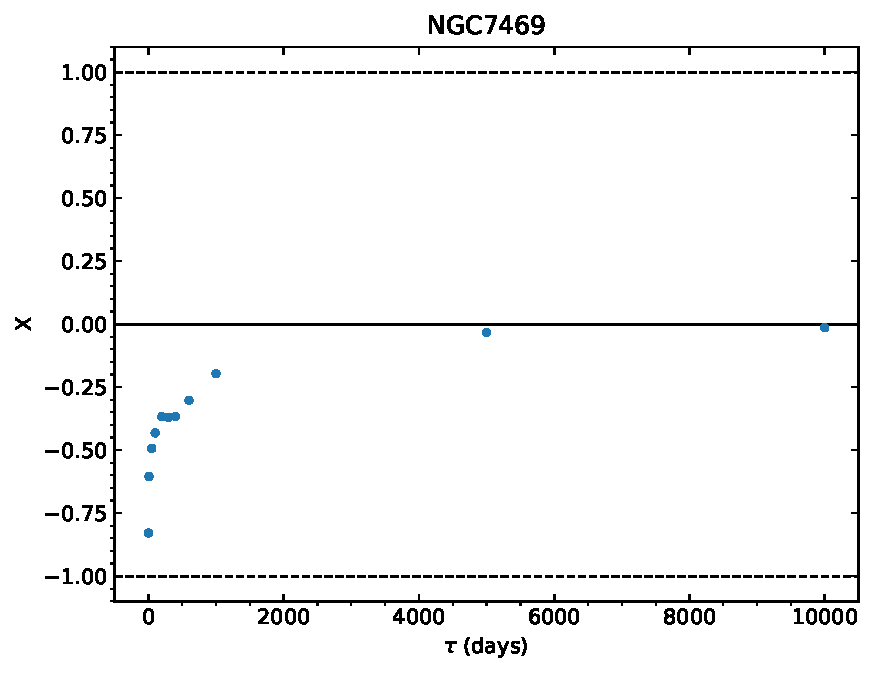
\includegraphics[width=0.49\textwidth]{Figs/Chapter5/X_tau/X_tau_NGC7469.pdf}  
  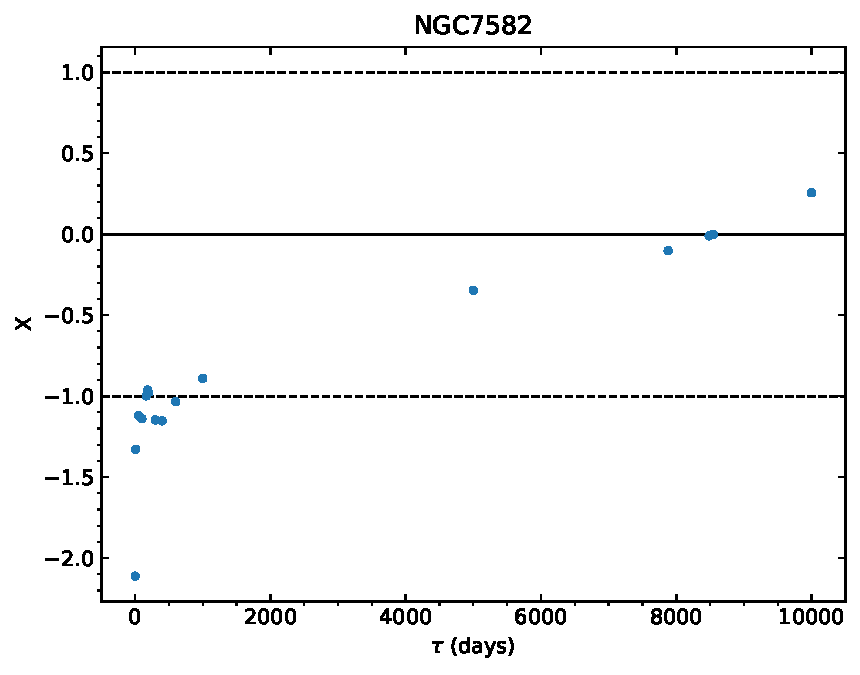
\includegraphics[width=0.49\textwidth]{Figs/Chapter5/X_tau/X_tau_NGC7582.pdf}  \hfill\\
  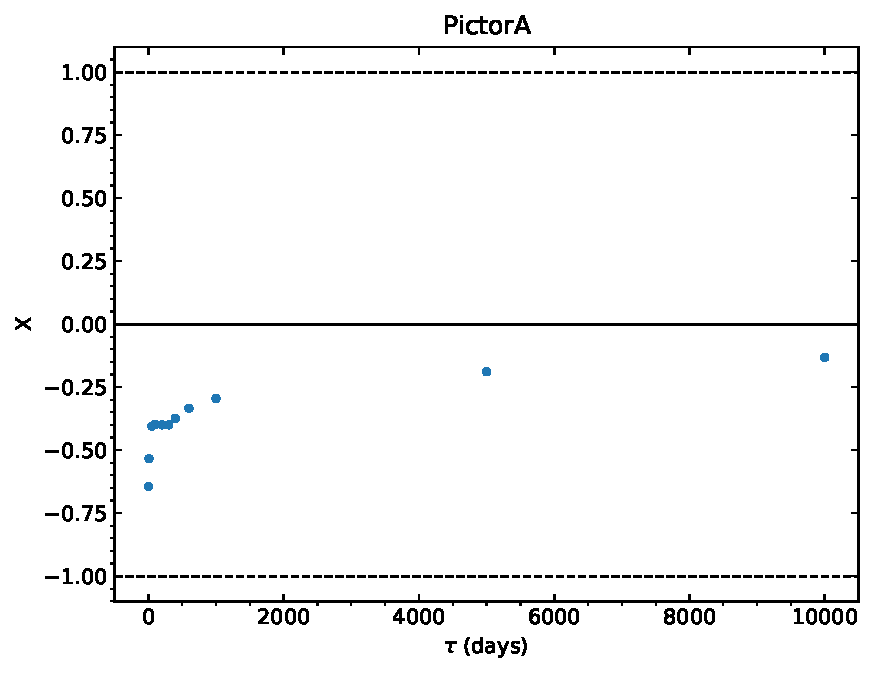
\includegraphics[width=0.49\textwidth]{Figs/Chapter5/X_tau/X_tau_PictorA.pdf}
  \caption{Fig.~\ref{fig:Xtau_1} continued.}
    \label{fig:Xtau_6}
  }
\end{center}
\end{figure}

